\documentclass[a4paper,10pt]{report}

\topmargin -2cm
%\topskip0cm
%\footskip0cm
%\headsep0cm
\parindent0cm
\oddsidemargin -1cm
\evensidemargin -1cm
\headheight 2cm
\textheight 24cm
\textwidth 18cm

\author{Daniel W\"aber (4049590)}
\title{\"Ubung}

\usepackage{ucs}
\usepackage[utf8x]{inputenc}
\usepackage{german}
\usepackage{color}
\usepackage{url}
\usepackage{graphicx}
\usepackage{algorithmic}

\pagestyle{empty}
\usepackage{makeidx}
\usepackage{amsmath}
\usepackage{amsfonts}
\usepackage{amssymb,euscript}
\usepackage{dsfont}
\usepackage{listings}
\usepackage{enumerate}
\newfont{\Fr}{eufm10}
\newfont{\Sc}{eusm10}
\newfont{\Bb}{msbm10}
\newcommand{\limin}{\lim_{n\rightarrow\infty}}
\newcommand{\limix}{\lim_{x\rightarrow\infty}}
\newcommand{\limun}{\lim_{n\rightarrow -\infty}}
\newcommand{\limux}{\lim_{n\rightarrow -\infty}}
\newcommand{\limx}{\lim_{x\rightarrow x_0}}
\newcommand{\limh}{\lim_{h\rightarrow 0}}
\newcommand{\defi}{\paragraph{Definition:}}
\newcommand{\bew}{\paragraph{Beweis:}}
\newcommand{\satz}{\paragraph{Satz:}}
\newcommand{\bsp}{\paragraph{Beispiel:}}
\newcommand{\lemma}{\paragraph{Lemma:}}
\newcommand{\N}{\mathds{N}}
\newcommand{\F}{\mathds{F}}
\newcommand{\Z}{\mathds{Z}}
\newcommand{\Q}{\mathds{Q}}
\newcommand{\R}{\mathds{R}}
\newcommand{\G}{\mathds{G}}
\newcommand{\C}{\mathds{C}}
\newcommand{\K}{\mathds{K}}
\newcommand{\A}{\mathds{A}}
\newcommand{\E}{\mathcal{E}}
\renewcommand{\P}{\mathcal{P}}
\newcommand{\sigA}{$\sigma$-Algebra }
\newcommand{\qed}{$\hfill\blacksquare$}
\newcommand{\arsinh}{\operatorname{arsinh} }
\newcommand{\arcosh}{\operatorname{arcosh} }
\newcommand{\gdw}{ $ \Leftrightarrow $ }
\newcommand{\tf}{ $ \Rightarrow $ }
\newcommand{\mgdw}{\Leftrightarrow}
\newcommand{\mtf}{\Rightarrow}
\newcommand{\Bild}{\text{Bild}}
\newcommand{\Kern}{\text{kern}}
\newcommand{\rg}{\text{rg}}
\newcommand{\deff}{\text{deff}}

\newcommand{\alphato}{\underset{\alpha}\to}
\newcommand{\betato}{\underset{\beta}\to}
\newcommand{\etato}{\underset{\eta}\to}
\newcommand{\ito}{\underset{i}\to}
\newcommand{\sto}{\underset{s}\to}
\newcommand{\kto}{\underset{k}\to}
\newcommand{\xto}{\underset{x}\to}

\usepackage{fancyhdr}
\pagestyle{fancy}
\lhead{Daniel Waeber\\Alex Muenn}
\chead{"Ubungsblatt \nr\\\today}
\rhead{Bildverarbeitung}


\newcommand{\nr}{6}
\lstset{language=matlab}

\begin{document}

\section*{Aufgabe 1 - Plot der Farbr\"aume}
Implementierung der Anforderung in wenigen Zeilen:
\begin{lstlisting}[language=matlab,caption=Approxiamation der vier neuen Pixel]
H = rgb2hsv(I);

plot3(I(:,:,1), I(:,:,2), I(:,:,3), '.');
plot3(H(:,:,1), H(:,:,2), H(:,:,3), '.');
\end{lstlisting}

Aus dem RGB-Diagramm geht f\"ur das menschliche Verst\"andnis die eigentliche
Farbverteilung besser hervor: Sehr viele dunkle Farbt\"one durch die Konzentration
um den Nullpunkt, geringe Farbdynamik durch lineare Verteilung (mit Ausnahme der 
zwei \"Aste f\"ur den grossen t\"urkisen und gelben Anteil) durch durch Grau/Weiss-Anteile. \\
Der Farbton l\"asst sich ohne Vorwissen von \texttt{Hue} aus dem HSV-Diagramm nicht
ableiten. Hier liegt der Vorteil in der Beschreibung der Farbt\"one. Im Diagramm ist
eine Verteilungswolke mit geringer S\"attigung  zu erkennen, die dem
dominierenden Schwarzton zuzuordnen ist. In der N\"ahe fallen zwei weitere Verteilungszentren mit wenig h\"oherer S\"attigung auf - Pastellton f\"ur das Spielfeld (Gr\"un) und das Tor (Gelb). Genrell ist das Bild relativ dunkel mit geringer Farbintensit\"at (viele Pixel mit geringer Helligkeit)

\begin{figure}[H]
\begin{center}
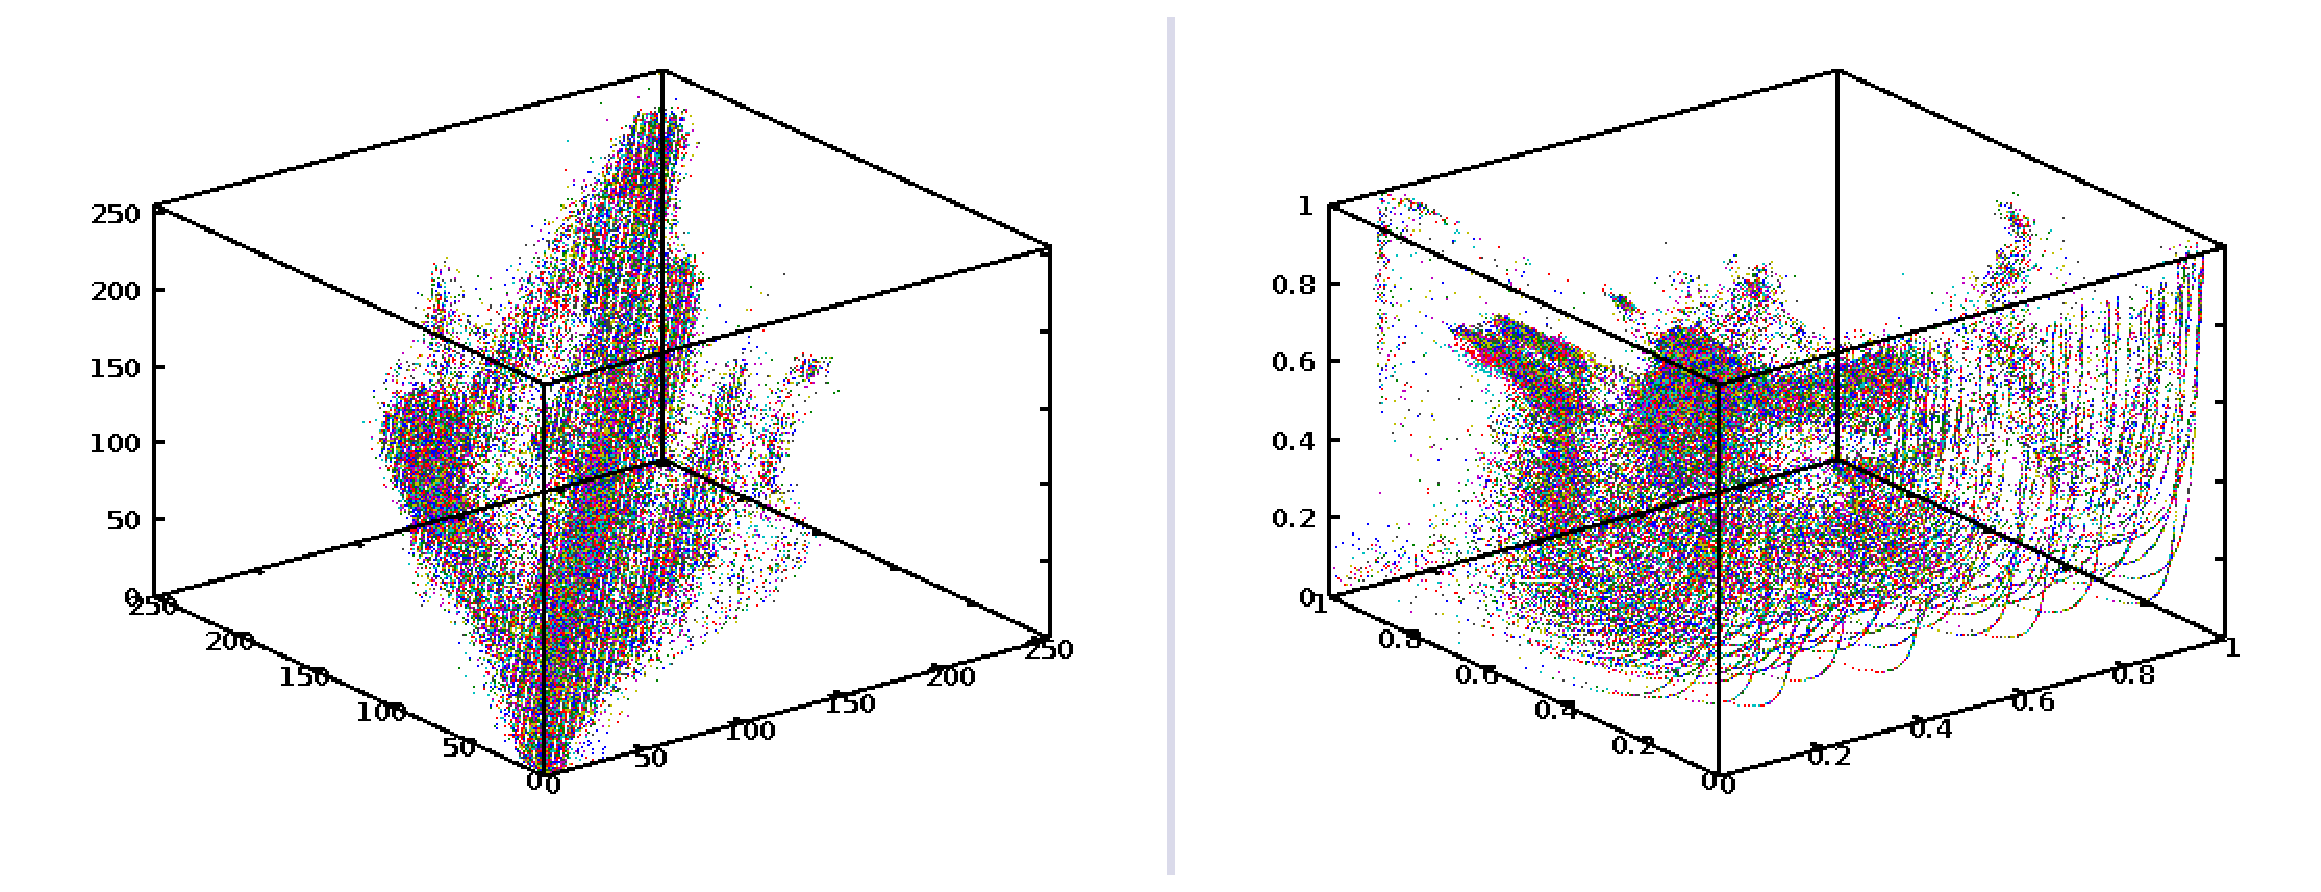
\includegraphics[width=100mm]{u08/graphs.eps}
\end{center}
\caption{Verteilung der Pixel im RGB-Farbraum (links) und HSV (rechts)}
\end{figure}



\section*{Aufgabe 2 - Farbersetzungen im RGB und HSV Farbraum}
\begin{itemize}
\item Bestimmung des Zielfarbtons in RGB ist z.B. $\vec{r} = [174,77,96]$ f\"ur 
      die Farbe des Torwart-Roboters
\item Betrachten der Farbinformation als Vektor
\item F\"ur jeden Pixel $\vec{p}$: Wenn $|laenge(\vec{p}-\vec{r})|< d$ dann
      wird die Farbe ersetzt
\item Im HSV-Farbraum analog, nur Farbwert und Distanz sind anzupassen
\end{itemize}

\begin{figure}[H]
\begin{center}
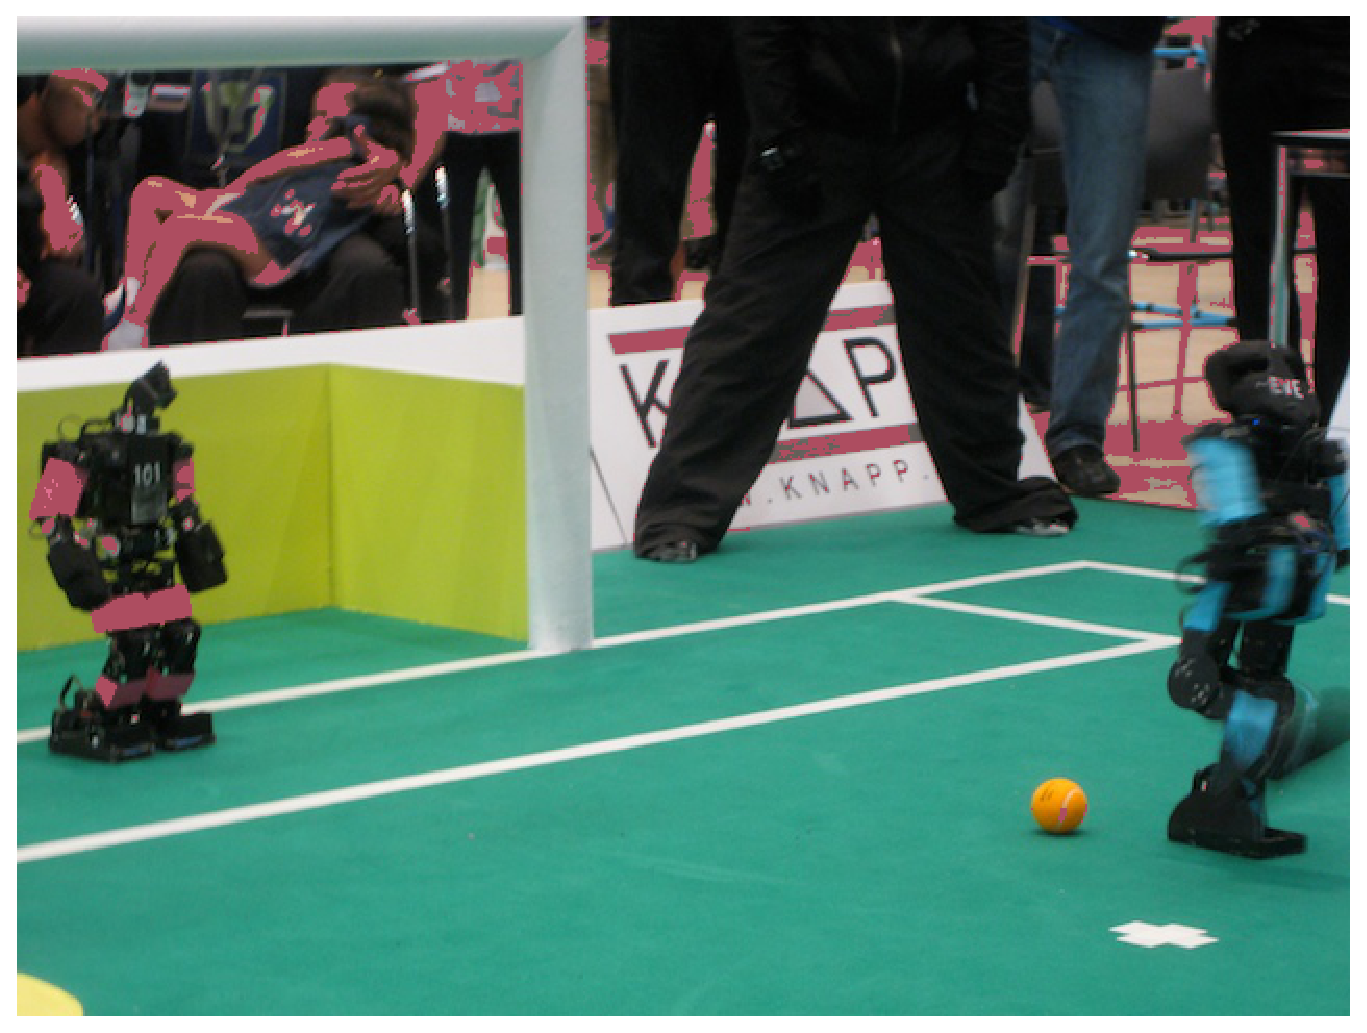
\includegraphics[width=100mm]{u08/dist_rgb.eps}
\end{center}
\caption{Uniformierung in RGB}
\end{figure}

\begin{figure}[H]
\begin{center}
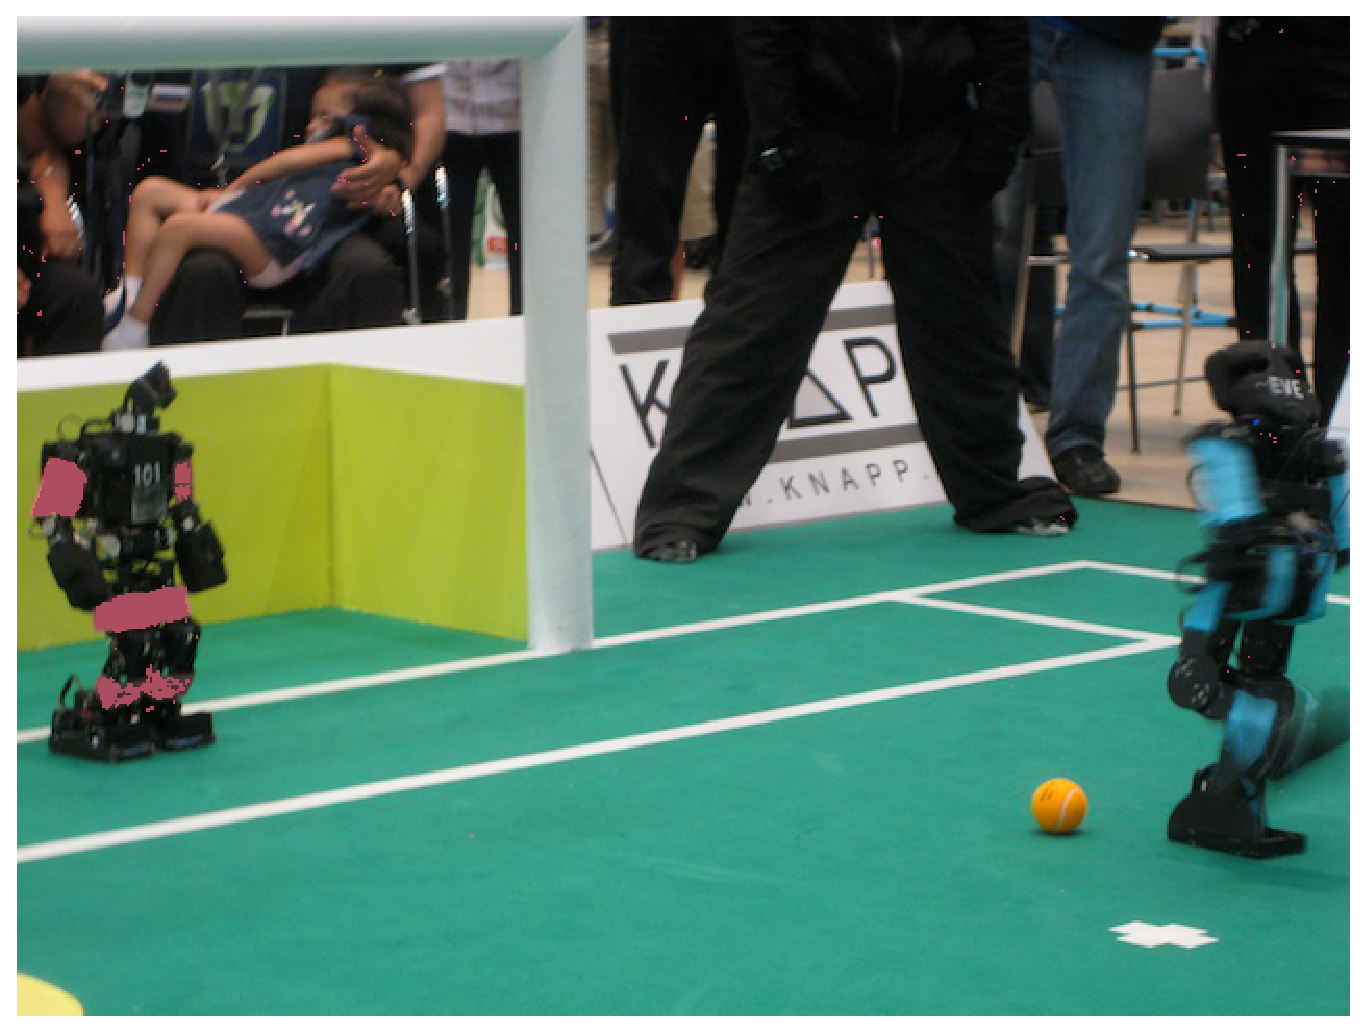
\includegraphics[width=100mm]{u08/dist_hsv.eps}
\end{center}
\caption{Bessere Uniformierung in HSW}
\end{figure}

Das Ergebnis der Ersetzung in HSV \"uberzeugt im Vergleich zur RGB-Variante. Ferner
war hier keine mehrmalige Nachjustierung n\"otig, um Qualit\"at des Ergebnisses zu
verbessern. \\
Begr\"unden l\"asst sich das damit, dass die tats\"achliche Farbcharakteristik in
HSV besser beschrieben wird und geringe Abweichung bereits gr\"ossere optische Fer\"anderung bewirken als im RGB-Raum.

\end{document}
